\documentclass{standalone}
\usepackage{graphicx}	
\usepackage{amssymb, amsmath}
\usepackage{color}

\usepackage{tikz}
\usetikzlibrary{shapes}
\usepackage{pgfmath}

\definecolor{light}{RGB}{220, 188, 188}
\definecolor{mid}{RGB}{185, 124, 124}
\definecolor{dark}{RGB}{143, 39, 39}
\definecolor{highlight}{RGB}{180, 31, 180}
\definecolor{gray10}{gray}{0.1}
\definecolor{gray20}{gray}{0.2}
\definecolor{gray30}{gray}{0.3}
\definecolor{gray40}{gray}{0.4}
\definecolor{gray60}{gray}{0.6}
\definecolor{gray70}{gray}{0.7}
\definecolor{gray80}{gray}{0.8}
\definecolor{gray90}{gray}{0.9}
\definecolor{gray95}{gray}{0.95}

\newcommand*{\h}{30}

\begin{document}

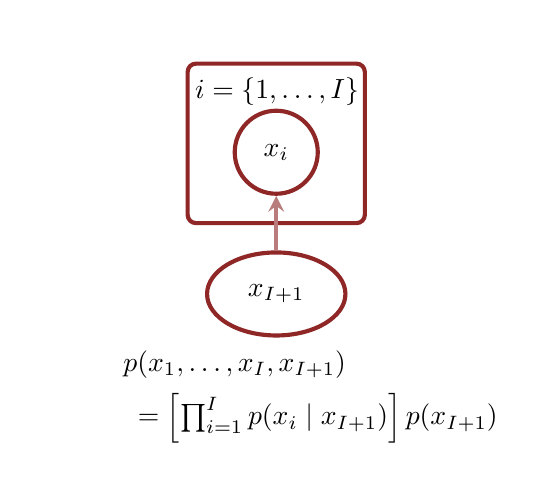
\begin{tikzpicture}[
   scale=0.15,
   obscirc/.style={circle, draw=dark, fill=dark, line width=1.5, text=white,
               inner sep=5, minimum size=\h},
   obsell/.style={ellipse, draw=dark, fill=dark, line width=1.5, text=white,
                  inner sep=5, minimum height=\h, minimum width=50},
   obsrec/.style={rectangle, draw=dark, fill=dark, line width=1.5, text=white,
                  inner sep=5, minimum height=\h, minimum width=\h},
   unobscirc/.style={circle, draw=dark, fill=white, line width=1.5, text=black,
                     inner sep=5, minimum size=\h},
   unobsell/.style={ellipse, draw=dark, fill=white, line width=1.5, text=black,
                    inner sep=5, minimum height=\h}, minimum width=50,
   unobsrec/.style={rectangle, draw=dark, fill=white, line width=1.5, text=black,
                    inner sep=1, minimum height=\h, minimum width=27},
   pushobscirc/.style={circle, draw=white, fill=dark, line width=1.5, dashed, text=white,
                    inner sep=1, minimum size=\h},
   pushunobscirc/.style={circle, draw=dark, fill=white, line width=1.5, dashed, text=black,
                    inner sep=1, minimum size=\h},
   pushell/.style={ellipse, draw=dark, fill=white, line width=1.5, dashed, text=black,
                   inner sep=1, minimum height=\h}
  ]

  % Node Spacing
  \pgfmathsetmacro{\d}{6}
  
  \begin{scope}[shift={(0, 0)}]
    \draw[white] (-3.5 * \d, -2.25 * \d) rectangle (3.5 * \d, 3.75 * \d);

    \draw[dark, rounded corners=3, line width=1.5] 
      (-1.25 * \d, 1 * \d) rectangle (+1.25 * \d, +3.25 * \d);
    \node[align=center] at (0.075 * \d, 2.85 * \d) { $i = \{ 1, \ldots, I \}$ };

    \node (A) at (0 * \d, 0 * \d) [unobsell] { $x_{I + 1}$ };
    
    %\node (B) at (-2.5 * \d, +2 * \d) [unobscirc] { $x_{1}$ };
    %\node (C) at (-1.25 * \d, +2 * \d) { $\ldots$ };
    \node (D) at (0 * \d, +2 * \d) [unobscirc] { $x_{i}$ };
    %\node (E) at (+1.25 * \d, +2 * \d)  { $\ldots$ };   
    %\node (F) at (+2.5 * \d, +2 * \d) [unobscirc] { $x_{K}$ };
    
    \foreach \B/\E in {A/D} {
      \draw[->, >=stealth, color=mid, line width=1.5] (\B) -- (\E);
    }
    
    \node[] at (0 * \d, -1 * \d) { $p( x_{1}, \ldots, x_{I}, x_{I + 1} ) \quad\quad\quad$ };
    \node[] at (0 * \d, -1.75 * \d) { $\quad\quad\quad = \left[ \prod_{i = 1}^{I} p( x_{i} \mid x_{I + 1} ) \right] p( x_{I + 1} )$ }; 

  \end{scope}

\end{tikzpicture}

\end{document}  